\documentclass[a4paper]{article}

\usepackage[svgnames]{xcolor}
\usepackage[UKenglish]{babel}
\usepackage[backend=bibtex,style=ieee]{biblatex}
\usepackage{booktabs}
\usepackage[font=small,format=plain,labelfont=bf,up,textfont=up]{caption}
\usepackage{fancyvrb}
\usepackage[margin=2cm]{geometry}
\usepackage{graphicx}
\usepackage{hyperref}
\usepackage{minted}
\usepackage{siunitx}
\usepackage{tikz}
\usepackage{todonotes} % Only for drafting
\usepackage{wrapfig}

\usetikzlibrary{positioning,shapes}

\addbibresource{d1report.bib}

% Args are module name, filename, caption text
% \newcommand{\modulelisting}[3]{
%   \begin{listing}[bp]
%     \linespread{.9}\inputminted[fontsize=\scriptsize,linenos]{systemverilog}{#2}
%     \caption{#3}
%     \label{lst:#1}
%   \end{listing}
% }
\newcommand{\modulelisting}[3]{
  \captionof{listing}{#3\label{lst:#1}}
  \linespread{.9}\inputminted[frame=single,fontsize=\scriptsize,linenos]{systemverilog}{#2}
  \vspace{20pt}
}

% Args are module name, caption text
\newcommand{\waveformfigure}[2]{
  \begin{figure}[bp]
    \centering\includegraphics[width=\textwidth]{assets/waveforms/#1}
    \caption{#2}
    \label{fig:wave:#1}
  \end{figure}
}

% Args are module name, caption text
\newcommand{\rtlfigure}[2]{
  \begin{figure}[bp]
    \centering\includegraphics[width=\textwidth]{assets/rtl/#1}
    \caption{#2}
    \label{fig:rtl:#1}
  \end{figure}
}

\setlength{\parindent}{0em}
\setlength{\parskip}{0.5em}

\title{ELEC2221 D1: Design and Test of a Sequential Multiplier}
\author{Kier Davis}

\begin{document}

\maketitle

\begin{table}[h]
  \centering
  \begin{tabular}{rl}
    Username: & kad2g15 \\
    Course: & MEng Electronic Engineering \\
    Tutor: & Dr. Klaus-Peter Zauner \\
    Lab group: & F17 \\
    Lab session: & 21st November 2016 \\
  \end{tabular}
\end{table}

%\todo[inline]{Write about Synplify optimising away the state machine due to the lack of a route from DONE back to IDLE}

\begin{abstract}
  A 4-bit unsigned sequential multiplier was implemented in SystemVerilog. The multiplier was thoroughly tested by preparing testbenches for each component of the multiplier, then simulating them in ModelSim. The design was synthesised for and downloaded onto a Lattice MachXO2 CPLD and tested manually. Finally, the multiplier was extended to operate on 8-bit numbers before being simulated and synthesised again.
\end{abstract}

\section{Implementation summary}
\label{sec:intro}

The algorithm implemented in the design is based on the one presented in \cite{gunton10}; however the add and shift operations are implemented together in a single clock cycle. The D1 sample code \cite{samplecode} was also referred to, as it uses a similar algorithm.

The design is broken down into separate modules, which are parameterised to allow easy configuration. In particular, the multiplier is parameterised by the width of its data input signals (4 bits, by default). This allows the design to be easily extended to larger operand sizes.

The design was tested by writing testbenches and simulating them in ModelSim. Assertions are used in the testbenches to automate checking the outputs for correctness.

\section{Adder design, simulation and synthesis}
\label{sec:adder}

The adder was implemented as part of the \texttt{multiplier\_datapath} module. It takes as inputs the current state of the \texttt{a} register and a signal named \texttt{addend}, and produces a 4-bit \texttt{sum} and a 1-bit \texttt{carry}. The value of \texttt{addend} is chosen based on the state of the least significant bit of \texttt{q}. If this bit is zero, \texttt{addend} is set to zero, and so the output of the adder is equal to \texttt{a}; that is, no actual addition is performed. If, however, the LSB of \texttt{q} is one, \texttt{addend} is set to \texttt{multiplicand}, and so the output of the adder is the sum of \texttt{a} and \texttt{multiplicand}.

\subsection{Implementation}
\label{sec:adder:impl}

The adder itself is implemented on line 72 of Listing~\ref{lst:multiplier_datapath}, and the multiplexer that produces \texttt{addend} is implemented on line 70.

\subsection{Simulation}
\label{sec:adder:sim}

The adder was not simulated on its own, but only as a part of \texttt{multiplier\_datapath}; see Section~\ref{sec:reg:sim} for further details.

It can be seen from the results of running the simulation of \texttt{multiplier\_datapath} in ModelSim (illustrated in Figure~\ref{fig:wave:test_multiplier_datapath}) that at the clock edge occurring at time \SI{8000}{\milli\second}, the value of the \texttt{product} signal changes from \texttt{0101~1001} to \texttt{1000~0100}. \texttt{product} is simply the concatenation of the \texttt{a} and \texttt{q} registers, so \texttt{a} must change from \texttt{0101} to \texttt{1000} and \texttt{q} must change from \texttt{1001} to \texttt{0100}. This is consistent with the results obtained by working through the method by hand:

\vspace{10pt}
\begin{tabular}{ll}
\mintinline{text}{  0101 1001} & Initial values of \texttt{a} and \texttt{q} \\
\mintinline{text}{+ 1011     } & Addend = multiplicand (\texttt{1011}), since LSB of \texttt{q} is 1 \\
\mintinline{text}{------     } & \\
\mintinline{text}{1 0000     } & \texttt{carry} and \texttt{sum} \\
\mintinline{text}{1 0000 1001} & Same as first line, but with \texttt{a} replaced by \texttt{carry} and \texttt{sum} \\
\mintinline{text}{  1000 0100} & Resulting of shifting previous line right by one place \\
\end{tabular}
\vspace{10pt}

This transition, and all other transitions of the \texttt{product} signal, are verified by assertions in the simulation. We can deduce that the adder is functioning correctly.

\section{Register design, simulation and synthesis}
\label{seg:reg}

The registers were implemented in the \texttt{multiplier\_datapath} module, together with the adder/shifter.

The \texttt{multiplier\_datapath} module has two 4-bit data inputs, \texttt{multiplicand} and \texttt{multiplier}. These are the two input numbers to the multiplier, and are equivalent to \texttt{M} and \texttt{Qin} respectively in the sample code. Similarly, there is one 8-bit data output, \texttt{product}, which is equivalent to \texttt{AQ} in the sample code \cite{samplecode}.

The module takes two control signals, \texttt{do\_init} and \texttt{do\_shift}, in addition to the clock and asynchronous reset signals. If \texttt{do\_init} is asserted during a rising clock edge, the \texttt{a} and \texttt{q} registers are loaded with their initial values (0 and \texttt{multiplier} respectively). If \texttt{do\_shift} is asserted during a rising clock edge, then \texttt{multiplicand} is conditionally added to \texttt{a}, and then \texttt{a} and \texttt{q} are shifted right by one place, completing one iteration of the multiplication algorithm.

\subsection{Implementation}
\label{sec:reg:impl}

The source code of the \texttt{multiplier\_datapath} module is given in Listing~\ref{lst:multiplier_datapath}.

\subsection{Simulation}
\label{sec:reg:sim}

A testbench for the \texttt{multiplier\_datapath} module was prepared. Its source code is given in Listing~\ref{lst:test_multiplier_datapath}. The testbench was then simulated using ModelSim, giving the waveform diagram shown in Figure~\ref{fig:wave:test_multiplier_datapath}. After correcting some minor syntax errors, the testbench and the module under test worked first time, without any assertions failing.

The testbench begins with the reset signal active, and checks that the registers \texttt{a} and \texttt{q} (whose values are concatenated to form the signal \texttt{product}) are reset to zero. It then releases the system from reset, and asserts the \texttt{do\_init} for one clock cycle, checking that \texttt{q} is set to 6, the value arbitrarily chosen for the second multiplier input. It then asserts \texttt{do\_shift} for four of the five following clock cycles, checking the state of the registers at each stage. The results of these operations can be observed in Figure~\ref{fig:wave:test_multiplier_datapath}.

\waveformfigure{test_multiplier_datapath}{Waveform of the \texttt{test\_multiplier\_datapath} testbench. Numbers shown in the waveform traces are in hexadecimal.}

% \subsection{Synthesis}
% \label{sec:reg:synth}

% The RTL generated for the \texttt{multiplier\_datapath} module during the synthesis process is shown in Figure~\ref{fig:rtl:multiplier_datapath}.

% \rtlfigure{multiplier_datapath}{Diagram of the synthesised RTL generated for the \texttt{multiplier\_datapath} module by Synplify Pro.}

\section{Sequencer design, simulation and synthesis}
\label{sec:seq}

The sequencer, an algorithmic state machine (ASM), is implemented in the \texttt{multiplier\_controller} module. It uses an auxillary 2-bit counter to store the number of remaining cycles of the shift/add operation. This counter has two control signal inputs, \texttt{do\_preset} and \texttt{do\_decrement}. \texttt{do\_preset} causes the counter to be set to its maximum value (3) on the next clock cycle, while \texttt{do\_decrement} causes the value of the counter to be decreased by 1 on the next clock cycle. It has only one output, \texttt{is\_zero}, which is high if the counter is equal to zero.

%\begin{wrapfigure}{r}{.5\textwidth}
\begin{figure}[bp]
  \centering
  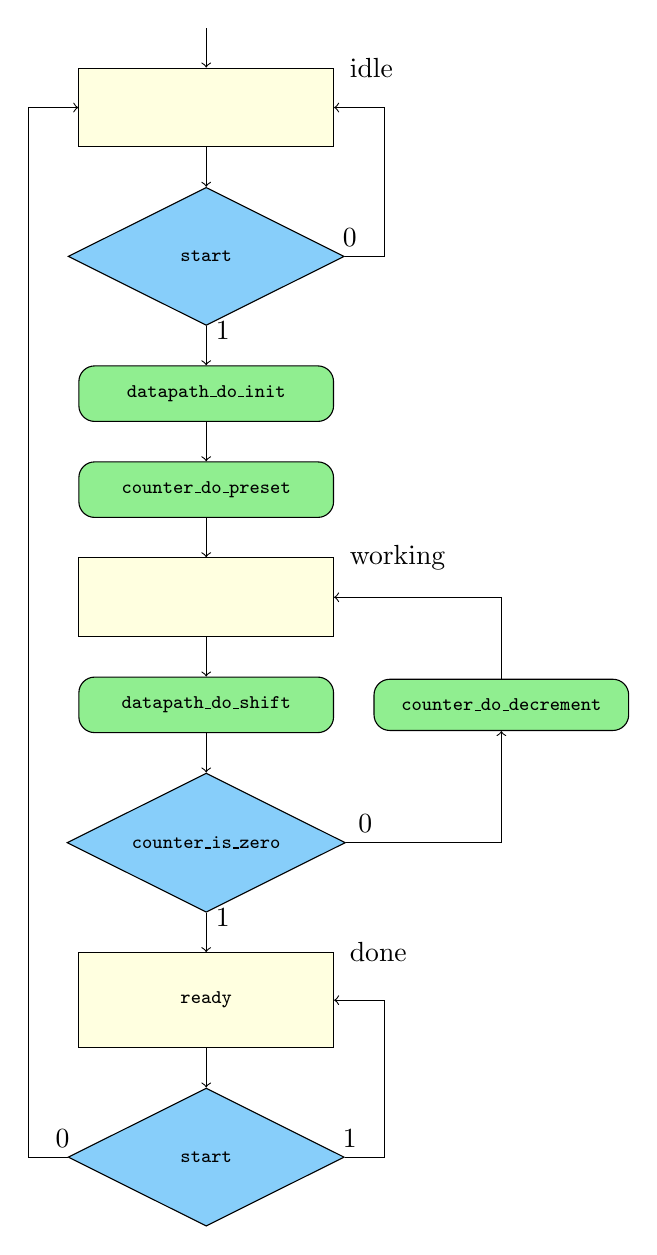
\begin{tikzpicture}[node distance=.5cm,
                    basenode/.style={draw,text width=3cm,text centered,inner ysep=.25cm,font={\scriptsize}},
                    state/.style={basenode,rectangle,inner ysep=.5cm,fill=LightYellow},
                    decision/.style={basenode,diamond,aspect=2,inner ysep=0cm,fill=LightSkyBlue},
                    condout/.style={basenode,rectangle,rounded corners=.2cm,fill=LightGreen}]
  \node[coordinate] (begin) {start};
  \node[state,label={[anchor=west,xshift=1.7cm]90:idle}] (idle) [below=of begin] {};
  \node[decision] (idle-start) [below=of idle] {\texttt{start}};
  \node[condout] (idle-datapath) [below=of idle-start] {\texttt{datapath\_do\_init}};
  \node[condout] (idle-counter) [below=of idle-datapath] {\texttt{counter\_do\_preset}};
  \node[state,label={[anchor=west,xshift=1.7cm]90:working}] (working) [below=of idle-counter] {};
  \node[condout] (working-datapath) [below=of working] {\texttt{datapath\_do\_shift}};
  \node[decision] (working-is-zero) [below=of working-datapath] {\texttt{counter\_is\_zero}};
  \node[state,label={[anchor=west,xshift=1.7cm]90:done}] (done) [below=of working-is-zero] {\texttt{ready}};
  \node[decision] (done-start) [below=of done] {\texttt{start}};
  \node[coordinate] (n1) [right=of idle-start] {};
  \node[coordinate] at (idle -| n1) (n0) {};
  \node[condout] (working-counter) [right=of working-datapath] {\texttt{counter\_do\_decrement}};
  \node[coordinate] at (working -| working-counter) (n2) {};
  \node[coordinate] at (working-is-zero -| working-counter) (n3) {};
  \node[coordinate] (n5) [right=of done-start] {};
  \node[coordinate] at (done -| n5) (n4) {};
  \node[coordinate] (n7) [left=of done-start] {};
  \node[coordinate] at (idle -| n7) (n6) {};
  \draw[->] (begin) -> (idle);
  \draw[->] (idle) -> (idle-start);
  \draw[->] (idle-start) -> node[right,very near start] {1} (idle-datapath);
  \draw[->] (idle-datapath) -> (idle-counter);
  \draw[->] (idle-counter) -> (working);
  \draw[->] (working) -> (working-datapath);
  \draw[->] (working-datapath) -> (working-is-zero);
  \draw[->] (working-is-zero) -> node[right,very near start] {1} (done);
  \draw[->] (done) -> (done-start);
  \draw[->] (idle-start) -- node[above,very near start] {0} (n1) -- (n0) -> (idle);
  \draw[->] (working-is-zero) -- node[above,very near start] {0} (n3) -> (working-counter);
  \draw[->] (working-counter) -- (n2) -> (working);
  \draw[->] (done-start) -- node[above,very near start] {1} (n5) -- (n4) -> (done);
  \draw[->] (done-start) -- node[above,very near start] {0} (n7) -- (n6) -> (idle);
\end{tikzpicture}
  \caption{An ASM chart outlining the operation of the multiplier. Rectangular nodes represent states, and arrows represent possible transition paths. The text inside each state node lists the unconditional outputs that are active during that state; the name of the state is instead given by the label at the top-right corner of the node. Rounded rectangles represent conditional outputs that should be asserted only when the transition path is taken. Diamonds represent decisions (input tests).}
  \label{fig:asm}
%\end{wrapfigure}
\end{figure}

The state machine, illustrated in Figure~\ref{fig:asm}, has three states named Idle, Working and Done. The system begins in the Idle state. When the \texttt{start} signal goes high, the system moves to the Working state. On this transition, the \texttt{a} and \texttt{q} registers are initialised by setting the datapath's \texttt{do\_init} signal high, and the counter is set to its maximum value by setting its \texttt{do\_preset} signal high.

While in the Working state, the datapath's \texttt{do\_shift} control input is held high, causing the \texttt{a} and \texttt{q} registers to be continually shifted and added. The state of the \texttt{is\_zero} signal is checked on each clock cycle; if it is high, then the system moves to the Done state, else it decreases the value of the counter by one by asserting the \texttt{do\_decrement} signal. Since \texttt{do\_shift} is still asserted when the counter's value is zero, it will be high for four clock cycles in a row, resulting in four iterations of the shift/add operation being applied to the \texttt{a} and \texttt{q} registers.

In the Done state, the system holds the \texttt{ready} output high, signalling the end of computation. It waits for the \texttt{start} input to go low again before transitioning back to the Idle state.

\subsection{Implementation}
\label{sec:seq:impl}

The 2-bit counter used for counting the number of remaining iterations of the shift/add operation is implemented in the \texttt{multiplier\_counter} module, whose source code is given in Listing~\ref{lst:multiplier_counter}. The remainder of the state machine is implemented in the \texttt{multiplier\_controller} module, whose source code is given in Listing~\ref{lst:multiplier_controller}.

\subsection{Simulation}
\label{sec:seq:sim}

A testbench for the counter was prepared; its source code is given in Listing~\ref{lst:test_multiplier_counter}. Running this testbench through ModelSim gives the waveform shown in Figure~\ref{fig:wave:test_multiplier_counter}. After cleaning up minor syntax errors, the simulation ran first time with all assertions passing.

The testbench begins with the reset input set to 0, resetting the counter to zero. At time \SI{2800}{\milli\second}, the \texttt{do\_preset} input is asserted, causing the count to be set to the maximum value (3) at the next clock edge (time \SI{3000}{\milli\second}). This signal is then de-asserted and the \texttt{do\_decrement} signal held high for three clock cycles. It can be observed that the count successfully decrements on each clock cycle that \texttt{do\_decrement} is held high for, eventually returning to zero. This behaviour is visible in the diagram.

\waveformfigure{test_multiplier_counter}{Waveform of the \texttt{test\_multiplier\_counter} testbench.}

Similarly, a testbench for the sequencer was also prepared. Listing~\ref{lst:test_multiplier_controller} gives the source code of this testbench, and Figure~\ref{fig:wave:test_multiplier_controller} shows the waveform produced by simulating the testbench in ModelSim. The testbench manipulates the \texttt{start} and \texttt{counter\_is\_zero} inputs to behave as if the system was performing multiplication. The controller can be seen to correctly assert \texttt{datapath\_do\_init} for one clock cycle, then \texttt{datapath\_do\_shift} for four clock cycles, as expected.

\waveformfigure{test_multiplier_controller}{Waveform of the \texttt{test\_multiplier\_controller} testbench.}

\subsection{Synthesis}
\label{sec:seq:synth}

Diagrams of the generated RTL logic for the counter and sequencer were extracted from the synthesis of the design and are presented in Figures~\ref{fig:rtl:multiplier_counter} and \ref{fig:rtl:multiplier_controller} respectively. The state machine at the core of the diagram for the sequencer has the transition diagram displayed in Figure~\ref{fig:fsm:diag} and the transition table shown in Figure~\ref{fig:fsm:tab}.

\rtlfigure{multiplier_counter}{Diagram of the synthesised RTL generated for the \texttt{multiplier\_counter} module by Synplify Pro.}

\rtlfigure{multiplier_controller}{Diagram of the synthesised RTL generated for the \texttt{multiplier\_controller} module by Synplify Pro.}

\begin{figure}[bp]
  \centering
  \begin{minipage}{.45\textwidth}
    \centering\includegraphics[width=.4\textwidth]{assets/rtl/fsm}
    \caption{State transition diagram generated for the \texttt{multiplier\_controller} module by Synplify Pro.}
    \label{fig:fsm:diag}
  \end{minipage}
  \hfill
  \begin{minipage}{.45\textwidth}
    \centering\begin{tabular}{lll}
      \toprule
      From state & To state & Condition \\
      \midrule
      \texttt{00} & \texttt{00} & \texttt{!start} \\
      \texttt{00} & \texttt{01} & \texttt{start} \\
      \texttt{01} & \texttt{01} & \texttt{!counter\_is\_zero} \\
      \texttt{01} & \texttt{10} & \texttt{counter\_is\_zero} \\
      \texttt{10} & \texttt{00} & \texttt{!start} \\
      \texttt{10} & \texttt{10} & \texttt{start} \\
      \bottomrule
    \end{tabular}
    \caption{State transition table generated for the \texttt{multiplier\_controller} module by Synplify Pro.}
    \label{fig:fsm:tab}
  \end{minipage}
\end{figure}

\section{Multiplier design, simulation and synthesis}
\label{sec:mult}

The \texttt{multiplier\_datapath}, \texttt{multiplier\_counter} and \texttt{multiplier\_controller} modules are encapsulated by the \texttt{multiplier} module, whose interface consists of the data inputs \texttt{multiplicand} and \texttt{multiplier}, the data output \texttt{product} and the control signals \texttt{start} and \texttt{ready}, as well as clock and asynchronous reset signals.

A seperate module, \texttt{machxo2\_pico\_frontend}, connects the multiplier's logical inputs and outputs to the hardware of the MachXO2 Pico board. This module creates instances of:
\begin{itemize}
  \item the multiplier itself
  \item the internal oscillator that produces the master clock
  \item the frequency divider that derives the multiplier's clock signal from the master clock
  \item the switch debouncer for the \texttt{start} button
\end{itemize}
Additionally, it defines the values of the multiplier's data inputs, \texttt{multiplicand} and \texttt{multiplier}. Since there are no physical switches available to control these inputs, they are hard-wired to constants. Values of 11 and 6 were arbitrarily chosen.

The internal oscillator is an instance of \texttt{OSCH} with a nominal frequency of \SI{4.16}{\mega\hertz}. The frequency divider, implemented in the \texttt{freq\_divider} module, uses a 22-bit counter to reduce this frequency to \SI{0.99}{\hertz}, allowing each step of the multiplication operation to be observed in real time.

The switch debouncer uses a simple counter to detect when the input becomes stable. Its behaviour is based on the implementation given in \cite{debouncer}: the counter is incremented by one for every consecutive clock cycle in which the input differs from the current output, and if the input returns to the same logic value as the output at any point, the counter is reset to zero. Once the counter reaches its maximum value, the input is assumed to have stopped oscillating, and so the current output state is updated to the same value as the input.

\subsection{Implementation}
\label{sec:mult:impl}

The source code of the \texttt{multiplier}, \texttt{freq\_divider}, \texttt{debouncer} and \texttt{machxo2\_pico\_frontend} modules is given in Listings~\ref{lst:multiplier}, \ref{lst:freq_divider}, \ref{lst:debouncer} and \ref{lst:machxo2_pico_frontend} respectively.

\subsection{Simulation}
\label{sec:mult:sim}

A testbench for the multiplier as a whole was written; its source code can be found in Listing~\ref{lst:test_multiplier}. Figure~\ref{fig:wave:test_multiplier} illustrates the result of running this testbench in ModelSim. It can be observed that an entire multiplication operation is completed in response to the \texttt{start} signal being brought high. The testbench contains assertions to check the values of \texttt{product} and \texttt{ready} at each clock cycle.

\waveformfigure{test_multiplier}{Waveform of the \texttt{test\_multiplier} testbench. Numbers shown in the waveform traces are in hexadecimal.}

Similarly, the \texttt{freq\_divider} module was also simulated in ModelSim. The testbench code is presented in Listing~\ref{lst:test_freq_divider}, producing the waveform shown in Figure~\ref{fig:wave:test_freq_divider}. For the purposes of simulation, the counter length was reduced from 22 bits to 8 bits, greatly reducing the length of time the simulation needs to run for. It can be seen that the output, \texttt{out\_clock}, has a much lower frequency than \texttt{in\_clock}. The testbench verifies through the use of assertions that the output frequency is $1/256$ the input frequency.

\waveformfigure{test_freq_divider}{Waveform of the \texttt{test\_freq\_divider} testbench.}

Finally, the \texttt{debouncer} was also simulated using the testbench displayed in Listing~\ref{lst:test_debouncer}. The testbench generates an input signal that oscillates rapidly at first, but decays in frequency over time. As demonstrated in Figure~\ref{fig:wave:test_debouncer}, the debouncer correctly smooths this signal to a single step.

\waveformfigure{test_debouncer}{Waveform of the \texttt{test\_debouncer} testbench.}

The \texttt{machxo2\_pico\_frontend} was not simulated as it depends on the built-in \texttt{OSCH} module, which is not available in external simulation tools such as ModelSim. Potentially, a simulatable drop-in replacement for \texttt{OSCH} could have been prepared, but \texttt{machxo2\_pico\_frontend} was not deemed to be complex enough to require this.

\subsection{Synthesis}
\label{sec:mult:synth}

The entire design was synthesised using Synplify Pro as part of the Lattice Diamond design flow. A block diagram of the system can be generated using the RTL netlist viewer; this is shown in Figure~\ref{fig:rtl:machxo2_pico_frontend}.

\rtlfigure{machxo2_pico_frontend}{Block diagram of the synthesised RTL generated for the top-level \texttt{machxo2\_pico\_frontend} module by Synplify Pro.}

A board containing 8 LEDs was wired up to the MachXO2 Pico board, and the synthesised design was then downloaded to the CPLD. As a result of the extensive simulation and testing of the components of the multiplier, the system worked on the CPLD without any changes being necessary.

\section{Extensions}
\label{sec:ext}

\subsection{8-bit datapath}
\label{sec:ext:8bit}

Once the main design had been synthesised and tested on the MachXO2 Pico board, the multiplier was extended to work with an operand width of 8 bits rather than 4. The modules are parameterised by the operand width (referred to as the parameter \texttt{N} in the source code), so implementing this extension was as simple as changing the value of \texttt{N} from 4 to 8, and adding an additional eight LED outputs to the system. The \texttt{machxo2\_pico\_frontend\_8bit} module, given in Listing~\ref{lst:machxo2_pico_frontend_8bit}, is a modified version of \texttt{machxo2\_pico\_frontend} with these changes applied.

A second LED board was wired up to the CPLD, and the design was re-synthesised and re-downloaded. At first glance it appeared that this design had produced an incorrect result: bit 7 of the product appeared to be low, while it was high in the result calculated by hand. However, it was observed that this LED did not light at any point during the multiplication process, and so it was determined that it was likely to be an electrical fault in the LED board or MachXO2 Pico board rather than a flaw in the SystemVerilog code.

\section{Conclusion}
\label{sec:con}

The project's goal, which was to design and implement a 4-bit sequential multiplier, was achieved. The multiplier was tested by simulating it in ModelSim, then synthesised onto a CPLD. The system was designed with a parameterisable data width, allowing it to be later increased to 8 bits with minimal change to the codebase.

The system could be further extended in a number of ways; examples include having data inputs controllable by a bank of DIP switches rather than being hardwired in the source code, or implementing the CORDIC algorithm, a similar shift-and-add based method for computing trigonometric and exponential functions.

Through this project, I gained experience of designing and implementing a moderately complex sequential system, and testing and synthesising this system using commerical CAD software.

\section{References}

\printbibliography[heading=none]

\clearpage
\section{Source code}

All source code is mirrored online at \url{https://github.com/kierdavis/multiplier}.

\modulelisting{multiplier_datapath}{../src/multiplier/multiplier_datapath.sv}
  {Source code of the \texttt{multiplier\_datapath} module, which contains the data registers $a$ and $q$ and the add/shift computation logic.}

\newpage

\modulelisting{test_multiplier_datapath}{../src/multiplier/test/test_multiplier_datapath.sv}
  {Source code of the \texttt{test\_multiplier\_datapath} module, which tests the operation of the data registers and add/shift computation logic.}

\modulelisting{multiplier_counter}{../src/multiplier/multiplier_counter.sv}
  {Source code of the \texttt{multiplier\_counter} module, which contains the 2-bit counter that records the number of remaining iterations of the algorithm.}

\modulelisting{test_multiplier_counter}{../src/multiplier/test/test_multiplier_counter.sv}
  {Source code of the \texttt{test\_multiplier\_counter} module, which tests the 2-bit counter used to keep track of the remaining number of iterations.}

\modulelisting{multiplier_controller}{../src/multiplier/multiplier_controller.sv}
  {Source code of the \texttt{multiplier\_controller} module, which contains the state machine that controls the multiplier's operation.}

\modulelisting{test_multiplier_controller}{../src/multiplier/test/test_multiplier_controller.sv}
  {Source code of the \texttt{test\_multiplier\_controller} module, which tests the operation of the state machine.}

\modulelisting{multiplier}{../src/multiplier/multiplier.sv}
  {Source code of the encapsulating module \texttt{multiplier}.}

\newpage

\modulelisting{test_multiplier}{../src/multiplier/test/test_multiplier.sv}
  {Source code of the \texttt{test\_multiplier} module, which tests the operation of the multiplier as a whole.}

\modulelisting{freq_divider}{../src/util/freq_divider.sv}
  {Source code of the \texttt{freq\_divider} module, which implements a divide-by-$2^{22}$ frequency divider.}

\modulelisting{test_freq_divider}{../src/util/test/test_freq_divider.sv}
  {Source code of the \texttt{test\_freq\_divider} module, which tests the frequency divider.}

\modulelisting{debouncer}{../src/util/debouncer.sv}
  {Source code of the \texttt{debouncer} module, which implements a simple switch debouncer for the start button.}

\modulelisting{test_debouncer}{../src/util/test/test_debouncer.sv}
  {Source code of the \texttt{test\_debouncer} module, which tests the start button debouncer.}

\modulelisting{machxo2_pico_frontend}{../src/frontends/machxo2_pico_frontend.sv}
  {Source code of the MachXO2 Pico frontend module \texttt{machxo2\_pico\_frontend}.}

\newpage

\modulelisting{machxo2_pico_frontend_8bit}{../src/frontends/machxo2_pico_frontend_8bit.sv}
  {Source code of the 8-bit version of the MachXO2 Pico frontend module \texttt{machxo2\_pico\_frontend\_8bit}.}

\end{document}
